%============================================================================
\section{Application of the Merger Tree Algorithm: Creating a Mock Galaxy Catalogue}
%============================================================================
\label{chap:mock_catalogues}

Now that we  know the optimal parameters to create  a merger tree with
\texttt{ACACIA}, we  use it to  generate a mock galaxy  catalogue.  We
summarize here the main data products generated by our code.
\begin{enumerate}
\item For  every snapshot of the  N body simulation, we  have the full
  clump catalogue  generated by \texttt{PHEW}. Every  clump is uniquely
  classified as a main halo or as a sub-halo.
\item Every dark  matter particle is given the clump  index it belongs
  to, or zero if it belongs to the smooth background.
\item For  each clump, we follow  and store the index  of the $n_{mb}$
  most strongly bound particles, the position of the density peak, the
  clump  bulk  velocities,  centre  of mass,  mass,  and  other  clump
  properties.
\item For each clump, we store the index of the direct progenitors (in
  particular its  main progenitor) and  its peak mass over  its entire
  past formation history.
\item We augment our clump database with orphan particles, storing for
  each of  them the index  of the last  known main progenitor  and its
  peak mass.
\end{enumerate}
To generate  the mock  galaxy catalogue,  we use  the well-established
technique of  Sub-Halo Abundance  Matching (SHAM). This  technique was
introduced  more than  ten  years  ago as  a  surprisingly simple  and
accurate  method  to  populate  a pure  dark  matter  simulation  with
galaxies  with the  correct  clustering statistics 
\citep{valeNonparametricModelLinking2006, shankarNewRelationshipsGalaxy2006, 
conroyModelingLuminositydependentGalaxy2006a}.


Although  several   implementations  of  SHAM  exist   in  the  recent
literature \citep{guoHowGalaxiesPopulate2010, 
wetzelWhatDeterminesSatellite2010, 
Moster2010, trujillo-gomezGalaxiesLCDMHalo2011, 
nuzaClusteringGalaxiesSDSSIII2013,
zentnerGalaxyAssemblyBias2014,
chaves-monteroSubhaloAbundanceMatching2016a} we use here  the variant 
based on the peak clump mass as a proxy for the stellar mass
\citep{reddickConnectionGalaxiesDark2013},          using          the
Stellar-Mass-to-Halo-Mass (SMHM) relation of \cite{Behroozi}.


Using the  peak clump mass  is believed  to mimick the  actual stellar
mass growth of a galaxy, first as a central galaxy when the host clump
was a main halo, then as a satellite galaxy when the halo was accreted
and became  a sub-halo.  After  infall, although the clump  mass might
decrease quickly due to interactions within the parent main halo, this
model assumes  that the  stellar mass in  the galaxy  remains constant
\citep{Nagai}.

Note that in  the SHAM methodology, the merger tree  algorithm plays a
central role.
\begin{enumerate}
\item In order to compute the clump peak mass, we need the entire mass
  growth past history.
\item  In order  to follow  galaxies even  when the  parent clump  has
  dissolved due  to numerical  overmerging, we  need to  follow orphan
  particles and their peak clump mass.
\end{enumerate}

Our parent DMO simulation uses $512^3 \simeq 1.3\times 10^8$ particles
and a box wize of 100 comoving  Mpc with a particle mass resolution of
$m_p \simeq  3.1 \times  10^8\msol$.  The cosmological  parameters are
taken from  the 2015 Planck Collaboration  results \citep{Planck2015},
with  Hubble constant  $H_0  = 67.74$  km s$^{-1}$Mpc$^{-1}$,  density
parameters  $\Omega_m  =  0.309$,  $\Omega_\Lambda  =  0.691$,  scalar
spectral index  $n_s = 0.967$,  and fluctuation amplitude  $\sigma_8 =
0.816$.  The initial conditions  were created using the \texttt{MUSIC}
code \citep{MUSIC}.   As explained  before, the density  threshold for
clump finding was  chosen to be 80 times the  mean background density,
$\bar{\rho} =  \Omega_m \rho_c$, and  the saddle threshold  for haloes
was set to  200$\bar{\rho}$, where $\rho_c = \frac{3  H_0^2}{8 \pi G}$
is the cosmological critical density.

As a  first application of our  merger tree code, we  will now compute
the two point correlation functions and the average radial profiles of
galaxy  clusters in  our simulation.  We will  compare our  results to
observational data, and demonstrate that  this is only when we include
orphan  galaxies  that   our  results  are  in   good  agreement  with
observations.

%============================================================================
\subsection{The Stellar Mass Correlation Function}\label{chap:correlation}
%============================================================================

\begin{figure}
  \centering
  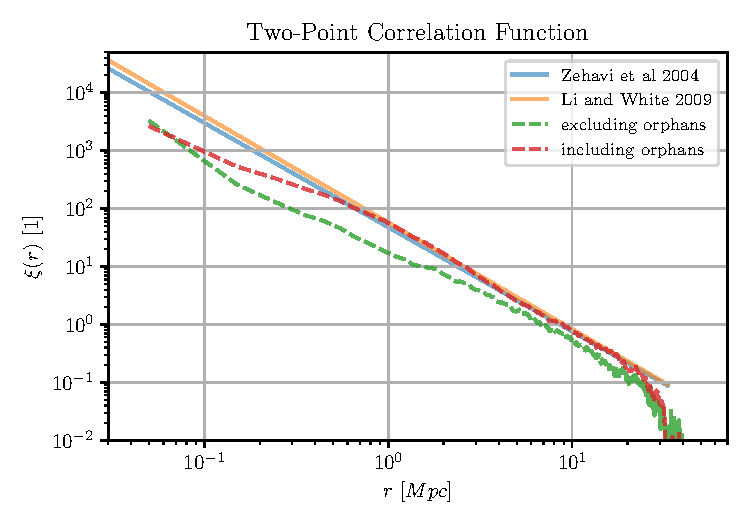
\includegraphics[width=\linewidth, keepaspectratio]{images/correlation.pdf}%
  \caption{The  predicted stellar  mass  2-point correlation  function
    (2PCF) $\xi(r)$ of our SHAM  model, including and excluding orphan
    galaxies, compared to  the power law fits of the  observed 2PCF in
    \citet{LiWhite} and \citet{Correlation1}.
  }%
  \label{fig:correlations}
\end{figure}

The  stellar mass  two-point correlation  function (2PCF)  $\xi(r)$ is
computed via  inverse Fourier transform  of the power  spectrum $P(k)$
\citep[e.g.][]{Mo},  which itself  can  be obtained  from the  Fourier
transform    of   the    stellar   mass    density   contrast    field
$\delta(\mathbf{r})$:
%
\begin{align}
  \delta_\mathbf{k} = \frac{1}{V}\int e^{i\mathbf{kr}} \delta(\mathbf{r}) \de ^3 \mathbf{r}
\end{align}
%
with
%
\begin{align}
	\delta(\mathbf{r}) = \frac{\rho(\mathbf{r})}{\langle \rho(\mathbf{r}) \rangle } - 1
\end{align}
%
Where $\rho(\mathbf{r})$ is the galaxy  stellar mass density field and
$\langle \rho(\mathbf{r}) \rangle$ is  the corresponding mean density,
$V = L^3$ is the volume of our large box on which the density field is
assumed  periodic,  and  $\mathbf{k}=\frac{2\pi}{L}(i_x,  i_y,  i_z)$,
where  $i_x,  i_y,  i_z$  are  integers.   The  Fourier  transform  is
performed using  the FFTW library \citep{FFTW05}.   The power spectrum
$P(k)$ and the 2PCF $\xi(r)$ are given by
%
\begin{align}
  P(k)    &= V \langle |\delta_\mathbf{k}|^2 \rangle \\
  \xi(r)  &= \frac{1}{(2\pi)^3} \int e^{-i\mathbf{kr}} P(k) \de^3 \mathbf{k} 
\end{align}
The simulation box is divided in  a uniform grid of $1024^3$ cells and
the  stellar mass  is  deposited  on the  grid  using a  cloud-in-cell
interpolation scheme.  The cloud-in-cell scheme consists  of assigning
each  galaxy a  cubic  volume  (``cloud'') the  size  of  a grid  cell
centered on the galaxy's position.  The galaxy stellar mass is assumed
to be uniformly distributed within the  cloud, and is deposited on the
uniform grid cells according to the  volume fraction of the cloud that
resides within each cell.

We only  include galaxies with  masses above $10^9 \msol$.   Using our
adopted SMHM relation,  these galaxies are hosted in  haloes with mass
larger than  $\sim 10^{11} \msol$,  or more than 300  particles.  This
threshold  ensures that  we  only  use well  resolved  clumps for  our
analysis, as discussed in the previous sections.

The predicted 2PCF $\xi(r)$ is shown in Figure \ref{fig:correlations},
and is  compared to  the observational  results of  \cite{LiWhite} and
\cite{Correlation1}.   Note  that  the observed  galaxy  catalogue  is
presented as  complete down  to $10^8 \msol$,  one order  of magnitude
smaller than our  simulated catalogue.  To highlight  the influence of
orphan galaxies,  we have  computed the predicted  2PCF both  with and
without  orphan  galaxies.   Including   orphan  galaxies  produces  a
correlation function in much  better agreement with observations.  Our
theoretical 2PCF obtained  reproduces the observed power  law fit over
two orders  of magnitude  in scale  of $r\sim 0.3  - 25$~Mpc.   On the
smallest  scales, below  0.3~Mpc,  our predictions  are  likely to  be
affected by our limited mass resolution and the grid resolution which 
is used for the Fourier Transform ($\sim 0.1$~Mpc per cell). We have 
verified that using a lower mass threshold for the stellar masses of 
galaxies makes no visible difference in the resulting correlation function.

The  role  of  the  orphan   galaxies  is  particularly  important  on
intermediate scales $\sim  0.2$ Mpc $<\ r \ <  2$ Mpc.  This behaviour
is explained by the fact that  orphan galaxies are located within host
haloes, thus contributing to the  correlations at small distances, the
so-called 1-halo term.  Our conclusion are in agreement  with those of
\cite{crisis}, who  have found that  the inclusion of  orphan galaxies
for mass-based SHAM models improves  the clustering statistics of mock
galaxy catalogues, particularly so at small scales.

%============================================================================
\subsection{Radial Profiles of Satellites in Large Clusters}\label{chap:radial-profiles}
%============================================================================

\begin{figure}
  \centering
  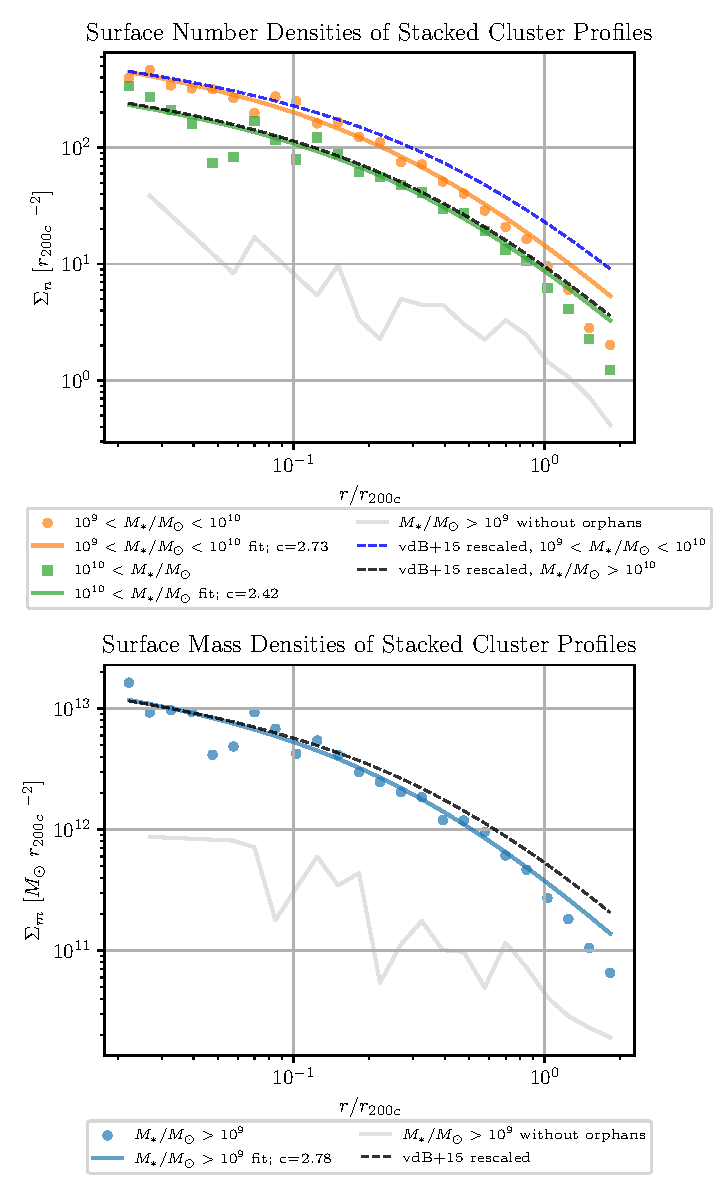
\includegraphics[width=\linewidth, keepaspectratio]{images/radial-profiles.pdf}%
  \caption{Upper panel: the light grey  solid line shows the satellite
    number density profile averaged over  the 10 largest haloes in our
    simulation {\it including only  satellite galaxies with a detected
    parent clump with masses above $10^9 \msol$}.   Satellites are  
    then grouped  in two  mass bins
    indicated in  the legend.   The colored  symbols show  the average
    number  density  profile  {\it  including  also  orphan  satellite
      galaxies}.  The colored solid  lines show the corresponding best
    fit projected NFW  profiles, while the  dashed lines  show the best  
    fit projected NFW profiles of the observed sample in
    \citet{vanderburgEvidenceInsideoutGrowth2015}.  Note  that for the
    latter,  we have  renormalized the  surface density  to match  the
    lower median mass of the  simulated sample (see text for details).
    The lower  panel shows the  stellar mass surface  density averaged
    over our  simulated sample. Here  again the light grey  solid line
    shows the  mass density profile  {\it only for  satellite galaxies
      within a detected  clump} while the blue symbols  shows the same
    quantity {\it also including  orphan satellite galaxies}. The blue
    solid  line corresponds  to our  best  fit projected NFW  profile while  the
    dashed line shows the best fit NFW profiles of the observed sample
    in \citet{vanderburgEvidenceInsideoutGrowth2015}.  Here again this
    last profile has  been renormalized to account  for the difference
    in  median mass  between the  simulated and  the observed  cluster
    samples.}
%
  \label{fig:radial-profiles}
\end{figure}

In this  section, we compute  the radial  profiles of number  and mass
densities  of satellite  galaxies in  the 10  largest clusters  in our
simulation. In  order to  compare to observations,  we will  follow as
closely      as     possible      the     method      described     in
\citet{vanderburgEvidenceInsideoutGrowth2015}, who analyzed 60 massive
clusters between 0.04<$z$<0.26 in  the Multi-Epoch Nearby Cluster Survey
and the Canadian Cluster Comparison Project.

We identified 10  haloes at $z=0$ with the highest  mass.  The mass is
defined here like  in \citet{vanderburgEvidenceInsideoutGrowth2015} as
$M_{200c}$, the  mass included within  radius $R_{200c}$ at  which the
average  enclosed  mass   density  of  the  halo  is   200  times  the
cosmological critical density $\rho_c$.   The $M_{200c}$ masses of our
10 selected  haloes range between  $1.4 \times 10^{14}\msol$  and $4.8
\times 10^{14}\msol$ with a median value of $1.6 \times 10^{14}\msol$.
Due to our limited box size, these  haloes are on the lower end of the
sample observed  in \citet{vanderburgEvidenceInsideoutGrowth2015}, who
reported masses ranging from $0.8 \times 10^{14}\msol$ and $1.6 \times
10^{15}\msol$ with a median value of $8.6 \times 10^{14}\msol$.

We compute  the projected number  density profiles and  projected mass
density  profiles as  follows: For  each  halo, we  first project  the
galaxies  (excluding the  central galaxy)  along each  coordinate axis
obtaining three  images.  We  then compute cylindrical  profiles using
radial shells equally space in log  radius in units of $r_{200c}$.  We
then average  the 30 profiles  (three projections for 10 clusters) to
obtain the final average radial surface density profile.  Each profile
is then fitted to a projected NFW profile \citep{navarroStructureColdDark1996b} using a
standard least square fitting procedure.   We obtain in particular the
concentration parameter that we can compare to the observed value.

The resulting profiles  are shown in Figure~\ref{fig:radial-profiles},
again including  and excluding  orphan galaxies. Orphan  galaxies play
here  also   a  crucial   role,  as   the  profiles   without  orphans
underestimate  the true  value by  an order  of magnitude.   Following
\citet{vanderburgEvidenceInsideoutGrowth2015},   we  adapt   the  same
galaxy  stellar   mass  $M_*$  thresholds   of  $10^9\msol  <   M_*  <
10^{10}\msol$ and $M_* > 10^{10}\msol$  for the surface number density
profile, and  a stellar mass threshold  of $M_* > 10^9  \msol$ for the
surface mass  density profile. It  is worth stressing that  this lower
mass threshold correspond exactly to  the mass resolution limit of our
mock galaxy catalogue.

As already noted above, the median  mass of the simulated and observed
catalogues  widely  differ.  In   order  to  facilitate  a  meaningful
comparison,  we  assume that  the  total  stellar mass  in  satellites
roughly  scales with  $M_{200c}$ in  the halo  mass range  of interest
here. We then adopt the following simple scaling relation
\begin{equation}
\Sigma \propto \frac{M_{200c}}{R_{200c}^2} \propto M_{200c}^{1/3}
\end{equation}
and    rescale    the    observed    average    profile    found    by
\citet{vanderburgEvidenceInsideoutGrowth2015}   using   this   scaling
relation  and  the  ratio  of  the  two  median  masses.  We  plot  in
Figure~\ref{fig:radial-profiles} the corresponding best fit projected NFW
profiles, showing excellent agreement with our simulated results.

Interestingly, the  observed surface density profiles  have a slightly
smaller concentration than  the simulated ones.  Although  we find for
the  number densities  of  satellite galaxies  above $10^{10}\msol$  a
concentration $c  = 2.4$,  in strikingly  good agreement  with $c=2.3$
found  by \citet{vanderburgEvidenceInsideoutGrowth2015}  for the  same
mass range, our results differ for the  mass range $10^9 \msol < M_* <
10^{10}        \msol$:       we        find       $c=2.7$        while
\citet{vanderburgEvidenceInsideoutGrowth2015} found  $c=1.8$. The same
mismatch is  found using the  mass density profile.  we  find $c=2.8$,
while \citet{vanderburgEvidenceInsideoutGrowth2015} found $c=2.0$.

We  believe  that this  mismatch  in  the concentration  parameter  is
consistent  with  the   difference  we  have  in   the  median  sample
mass. Indeed, the  theory predicts a larger  concentration for smaller
mass haloes, roughly in the amplitude observed here \citep{zhaoAccurateUniversalModels2009}. 
We therefore  could in principle improve the agreement
between   our    simulation   results   and   the    observations   of
\citet{vanderburgEvidenceInsideoutGrowth2015}  by  also rescaling  the
radial direction according to the theoretical expectations. We believe
this is  beyond the  scope of this  paper to try  and fit  exactly the
data.

In   addition,    we   believe   there    is   much   more    to   the
story. \citet{vanderburgEvidenceInsideoutGrowth2015} found that larger
mass  satellite galaxies  have  a  significantly larger  concentration
parameter   than    the   low   mass   bin    ($c=2.3$   compared   to
$c=1.8$). Moreover, they have also  found a strong excess of satellite
galaxies compared to the best fit NFW  profile in the centre ($r < 0.1
R_{200c}$).   These observations  are  consistent with  the effect  of
dynamical friction  bringing the more  massive galaxies faster  to the
central regions of  the cluster. Dynamical friction is  expected to be
sufficiently efficient  for the  most massive  sub-haloes, with  a mass
larger than a few  percent of that of the host  halos 
\citep[e.g.][]{binneyGalacticDynamicsSecond2008,Mo}. 
In our case, this  translates into
sub-haloes  more  massive  than  a  few  $10^{12}\msol$  and  satellite
galaxies  more  massive than  a  few  $10^{10}\msol$.  Our  simulation
clearly suffers from  numerical overmerging in this  mass range 
\citep{vandenboschDisruptionDarkMatter2018}, as highlighted  by the 
importance of including  orphan galaxies in
our  methodology.  Moreover,  our  pure DMO  parent simulation  cannot
follow precisely the many baryonic  effects that are needed to predict
accurately the  individual trajectory  of these higher  mass satellite
galaxies.

With these  caveats in mind,  we conclude  that using our  merger tree
code and a  state-of-the-art SHAM method, we can  model reasonably well
the cluster satellite galaxy number density and mass density profiles.
